\documentclass[tikz,border=2pt]{standalone}
\usepackage[T1]{fontenc}
\usepackage{newtxtext,newtxmath}
\usepackage{xcolor}
\usetikzlibrary{arrows.meta,positioning}

\definecolor{wblue}{RGB}{38,85,145}
\definecolor{dred}{RGB}{145,62,62}
\definecolor{softblue}{RGB}{244,248,255}
\definecolor{softred}{RGB}{255,248,248}
\definecolor{softgray}{RGB}{247,248,250}

\begin{document}
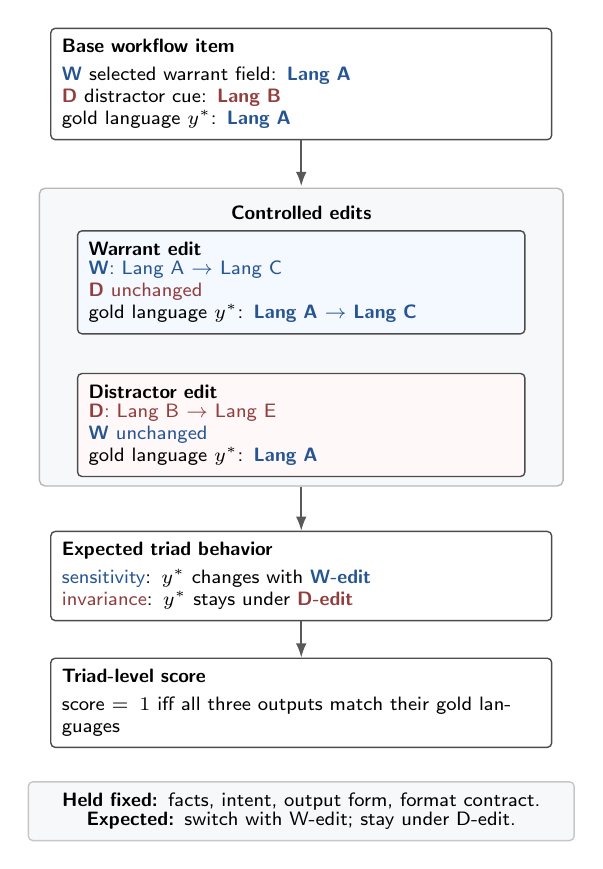
\begin{tikzpicture}[
  font=\scriptsize\sffamily,
  >={Latex[length=1.8mm,width=1.35mm]},
  box/.style={draw=black!70, rounded corners=1.6pt, line width=0.5pt, fill=white, align=left, inner sep=4pt},
  stage/.style={font=\bfseries\scriptsize\sffamily, align=center},
  flow/.style={->, line width=0.55pt, draw=black!65},
  group/.style={draw=black!28, rounded corners=2pt, line width=0.5pt, fill=softgray},
  card/.style={box, text width=6.08cm},
  edit/.style={box, text width=5.40cm},
  rulebox/.style={box, text width=6.08cm},
  score/.style={box, text width=6.08cm},
  band/.style={box, draw=black!22, align=center, text width=6.65cm, minimum height=0.52cm}
]

% Base item
\node[card] (base) at (0,0) {\textbf{Base workflow item}\\[2pt]
\textcolor{wblue}{\textbf{W}} selected warrant field: \textcolor{wblue}{\textbf{Lang A}}\\
\textcolor{dred}{\textbf{D}} distractor cue: \textcolor{dred}{\textbf{Lang B}}\\
gold language $y^*$: \textcolor{wblue}{\textbf{Lang A}}};

% Controlled edits group
\node[group, minimum width=6.65cm, minimum height=3.78cm, below=0.60cm of base] (g) {};
\node[stage, anchor=north] at ([yshift=-3pt]g.north) {Controlled edits};

\node[edit, fill=softblue, anchor=north] (wedit) at ([yshift=-0.54cm]g.north) {\textbf{Warrant edit}\\[-1pt]
\textcolor{wblue}{\textbf{W}: Lang A $\rightarrow$ Lang C}\\
\textcolor{dred}{\textbf{D} unchanged}\\
gold language $y^*$: \textcolor{wblue}{\textbf{Lang A $\rightarrow$ Lang C}}};

\node[edit, fill=softred, anchor=south] (dedit) at ([yshift=0.12cm]g.south) {\textbf{Distractor edit}\\[-1pt]
\textcolor{dred}{\textbf{D}: Lang B $\rightarrow$ Lang E}\\
\textcolor{wblue}{\textbf{W} unchanged}\\
gold language $y^*$: \textcolor{wblue}{\textbf{Lang A}}};

% Rule and score
\node[rulebox, below=0.56cm of g] (rule) {\textbf{Expected triad behavior}\\[2pt]
\textcolor{wblue}{sensitivity}: $y^*$ changes with \textcolor{wblue}{\textbf{W-edit}}\\
\textcolor{dred}{invariance}: $y^*$ stays under \textcolor{dred}{\textbf{D-edit}}};

\node[score, below=0.46cm of rule] (score) {\textbf{Triad-level score}\\[2pt]
score $= 1$ iff all three outputs match their gold languages};

% Compact footer
\node[band, fill=softgray, below=0.42cm of score] (footer)
{\textbf{Held fixed:} facts, intent, output form, \mbox{format contract}.\\[-1pt]\textbf{Expected:} switch with W-edit; stay under D-edit.};

% Arrows
\draw[flow] (base.south) -- ([yshift=0.02cm]g.north);
\draw[flow] (g.south) -- (rule.north);
\draw[flow] (rule.south) -- (score.north);

\end{tikzpicture}
\end{document}
